\subsection{Flutuações de energia}\label{sec:5.2}
Hora de examinar os efeitos da emissão quântica sobre as oscilações de energia de um elétron armazenado. Quando uma quantidade de energia é emitida, a energia do elétron subitamente decresce de uma quantidade $u$. Este distúrbio impulsivo causa uma pequena oscilação de energia. O efeito cumulativo de várias distorções -- ocorrendo em tempos aleatórios -- faz com que a oscilação de energia cresça (como em um caminho aleatório). O crescimento é limitado -- na média -- pelo amortecimento; e, em condições estacionárias, as oscilações de energia de um elétron em particular irão flutuar em torno de uma amplitude média. Estas flutuações de energia serão analisadas agora.

Em um primeiro momento, apenas será considerada a medida típica da oscilação de energia -- ou seja, a raiz quadrada média do desvio da energia média -- sem considerar detalhadamente a distribuição de probabilidade do desvio de energia. A natureza desta distribuição será considerada depois.

Na \autoref{sec:3.5} foram analisadas as pequenas oscilações do desvio de energia de um elétron armazenado. Na ausência de distúrbios, e ignorando por agora o amortecimento, o desvio de energia $\epsilon$ é descrito por
\begin{align}
	\epsilon = A_0 e^{i\Omega(t-t_0)}
\end{align}
onde $\Omega$ é a frequência síncrotron (real) e a amplitude $A_0$ é um número real. Agora, suponha que em algum instante $t_i$ a energia subitamente decresça de uma quantidade $u$ -- por emissão quântica. Depois de $t_i$ a energia será como
\begin{align}
	\epsilon = A_0 e^{i\Omega(t-t_0)} - ue^{i\Omega(t-t_i)}
\end{align}
Veja a \autoref{fig:fig43}. Esta nova oscilação pode ser escrita como
\begin{align}
	\epsilon = A_1e^{i\Omega(t-t_1)}
\end{align}
onde
\begin{align}
	A_1^2 = A_0^2 + u^2 - 2A_0u\ cos(\Omega (t_i-t_0))
\end{align}
e $t_1$ é algum deslocamento de tempo que não importa agora.

\begin{figure}[!htb]
	\centering
	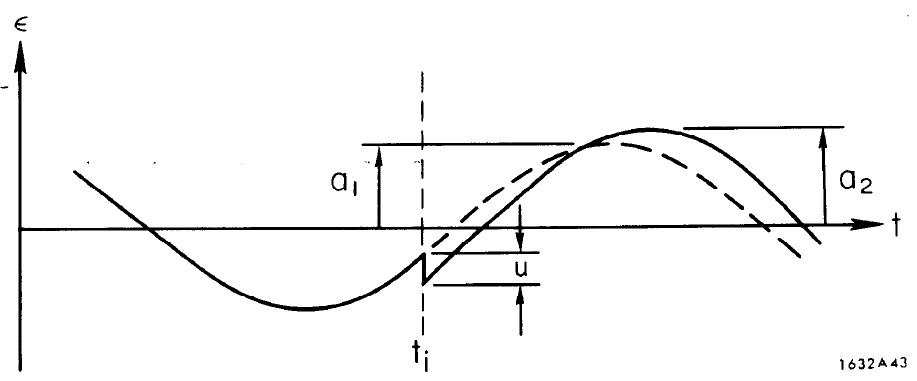
\includegraphics[width=0.9\linewidth]{./Figuras/fig43.jpeg}
	\caption{Efeito nas oscilações de energia devido à emissão de uma quantidade de energia $u$. Retirado de \cite{sands1970physics}.}
	\label{fig:fig43}
\end{figure}

\begin{proof}
	Seja $\epsilon$ dado por
	\begin{align*}
		\epsilon = A_0 e^{i\Omega(t-t_0)} - ue^{i\Omega(t-t_i)}
	\end{align*}
	Fazendo o produto dele pelo seu conjugado, tem-se que
	\begin{align*}
		\epsilon \epsilon^* &= [A_0 e^{i\Omega(t-t_0)} - ue^{i\Omega(t-t_i)}][A_0 e^{-i\Omega(t-t_0)} - ue^{-i\Omega(t-t_i)}]\\
							&= A_0^2 + u^2 - A_0 u[e^{i\Omega(t_i-t_0)} + e^{-i\Omega(t_i-t_0)}]
	\end{align*}
	Pela fórmula de Euler, pode-se transformar as exponencias em senos e cossenos:
	\begin{align*}
		e^{i\Omega(t_i-t_0)} + e^{-i\Omega(t_i-t_0)} &= cos(\Omega(t_i-t_0)) + i\ sen(\Omega(t_i-t_0)) + cos(-\Omega(t_i-t_0)) + i\ sen(-\Omega(t_i-t_0))\\
		&= 2cos(\Omega(t_i-t_0))
	\end{align*}
	Logo,
	\begin{align*}
		\epsilon \epsilon^* = A_0^2 + u^2 - 2A_0u\ cos(\Omega(t_i-t_0))
	\end{align*}
	Agora, deseja-se escrever $\epsilon$ na forma $A_1e^{i\Omega(t-t_1)}$. A partir desta definição, pode-se novamente realizar o produto de $\epsilon$ pelo seu conjugado:
	\begin{align*}
		\epsilon \epsilon^* &= A_1^2\\
		\therefore A_1^2 = A_0^2 + u^2 &- 2A_0u\ cos(\Omega(t_i-t_0))
	\end{align*}
	c.q.d.
\end{proof}

A emissão quântica altera a amplitude da oscilação para um novo valor que depende da amplitude inicial e de $(t_i-t_0)$. Já que o tempo $t_i$ onde uma emissão quântica ocorre é totalmente imprevisível -- e apenas o efeito cumulativo destes eventos interessa -- apenas questões estatísticas são relevantes. Por exemplo: qual a provável mudança de amplitude? Em geral, a fase $(t_i-t_0)$ é completamente aleatória e o valor esperado de $cos(\Omega(t_i-t_0))$ é, portanto, zero. Então a mudança de amplitude provável devido à radiação quântica é
\begin{align}
	\mean{\delta A^2} = \mean{A_1^2 - A_0^2} = u^2
\end{align}
Note que este resultado diz que a mudança provável em $A^2$, a qual ocorre quando é adicionado um novo incremento de oscilação de amplitude $u$ com fase aleatória, é apenas $u^2$ -- o mesmo resultado que seria obtido para $\delta A^2$ se a análise tivesse começado com $A=0$.

Suponha agora que estes eventos quânticos ocorrem em uma sequência de tempo aleatória com uma taxa média $\mathscr{N}$ (número por unidade de tempo). Cada evento muda $A^2$ por uma quantidade $u^2$; e, já que o tempo médio entre cada evento é $1/\mathscr{N}$, espera-se que
\begin{align}
	\mean{\frac{dA^2}{dt}} = \mathscr{N}u^2
\end{align}
Mas a provável taxa de variação de $A^2$ é igual a taxa de variação do valor provável de $A^2$, então
\begin{align}
	\frac{d\mean{A^2}}{dt} = \mathscr{N}u^2\label{eq:5.27}
\end{align}

Além de excitar as oscilações de energia, as perdas de energia discretas contribuem para uma mudança cumulativa na energia. No entanto, estes efeitos médios já foram considerados anteriormente. Seu efeito é produzir as oscilações de energia bem como causar o amortecimento exponencial da amplitude $A$ com uma constante de tempo $\tau_\epsilon = 1/\alpha_\epsilon$. Com este amortecimento, a amplitude decresce a uma taxa $A/\tau_\epsilon$; ou seu quadrado com uma taxa $2A^2/\tau_\epsilon$. A amplitude provável deve ser decrescida pelo amortecimento de forma similar, o que contribuiria à taxa de variação de $\mean{A^2}$ a quantidade
\begin{align}
	\frac{d\mean{A^2}}{dt} = -2\frac{\mean{A^2}}{\tau_\epsilon}\label{eq:5.28}
\end{align}
Quando tanto a excitação quântica quanto o amortecimento estão agindo -- e outras condições estão em estado estacionário -- a soma das taxas das equações \eqref{eq:5.27} e \eqref{eq:5.28} deve ser zero. Logo, encontra-se que o valor provável de $A^2$ é dado por
\begin{align}
	\mean{A^2} = \frac{1}{2}\tau_\epsilon \mathscr{N}u^2
\end{align}
Para oscilações de energia senoidais, o valor esperado de $\epsilon$ é zero, e do seu quadrado -- o qual pode-se chamar de $\sigma_\epsilon^2$ -- é apenas $1/2$ vezes o valor provável do quadrado da amplitude:
\begin{align}
	\sigma_\epsilon^2 = \mean{\epsilon^2} = \frac{\mean{A^2}}{2} = \frac{1}{4}\tau_\epsilon \mathscr{N} u^2\label{eq:5.30}
\end{align}
Desta forma, seria a média do quadrado da flutuação de energia na oscilação de energia que seria produzida pelas emissões quânticas aleatórias, todas de mesma energia $u$. Isto deve corresponder aproximadamente às flutuações de energia em um anel de armazenamento se $u$ fosse a energia quântica típica $u_c$ e $\mathscr{N}$ fosse a taxa média $P_\gamma/u_c$.

Um resultado equivalente aproximado pode ser obtido a partir de um simples argumento. A flutuação de energia típica vem do desvio da média do número de quantidade de energia emitida em um intervalo de amortecimento $\tau_\epsilon$. A média do número emitido é $\mathscr{N}\tau_\epsilon$, então o desvio RMS da média é $\sqrt{\mathscr{N}\tau_\epsilon}$ (distribuição de Poisson). Já que cada partícula quântica tem energia em torno de $u_c$, na média,
\begin{align}
	\sigma_\epsilon \approx \sqrt{\mathscr{N}\tau_\epsilon}u_c
\end{align}
Este resultado é parecido com o que foi obtido na equação \eqref{eq:5.30}. Note que, como $\mathscr{N} \approx P_\gamma/u_c$ e $\tau_\epsilon \approx E_0/P_\gamma$, também pode-se escrever
\begin{align}
	\sigma_\epsilon \approx \sqrt{E_0 u_c}\label{eq:5.32}
\end{align}
Concluindo: a flutuação de energia é aproximadamente a média geométrica entre a energia do elétron e a energia crítica do fóton!

Pode-se, então, fazer um cálculo mais preciso -- o qual é um pouco mais complicado. Primeiro, porque existe uma distribuição estatística do tamanho das quantidades de energia. Segundo, porque tanto a distribuição quanto a taxa média podem variar ao longo do anel. Retornando à equação \eqref{eq:5.27}, deve-se considerar separadamente a contribuição de cada intervalo de tamanhos quânticos a $d\mean{A^2}/dt$. Estas quantidades com energias entre $u$ e $u+\Delta u$ -- onde existem $n(u)\Delta u$ quantidades de energia emitidas por unidade de tempo -- irão contribuir com
\begin{align}
	\Delta \left\{\frac{d\mean{A^2}}{dt}\right\} = u^2 n(u) \Delta u
\end{align}
Mas como a emissão quântica em várias energias não são correlacionadas, cada energia irá contribuir de forma independente ao crescimento aleatório de $\mean{A^2}$. Então basta somar as contribuições de cada intervalo $\Delta u$:
\begin{align}
	\frac{d\mean{A^2}}{dt} = \int\limits_{0}^{\infty}u^2n(u)du
\end{align}
Esta integral já foi analisada: é apenas $\mathscr{N}\mean{u^2}$ (equação \eqref{eq:5.17}). Logo,
\begin{align}
	\frac{d\mean{A^2}}{dt} = \mathscr{N}\mean{u^2}
\end{align}

A taxa de crescimento obtida depende da energia do elétron -- a qual pode ser avaliada como a energia nominal $E_0$ -- e do raio local de curvatura da trajetória $\rho$, ambos os quais podem variar ao longo do anel. Da derivação feita, pode-se esperar que o tempo para haver uma variação "significante" na amplitude da oscilação de energia será da ordem da constante de tempo de amortecimento $\tau_\epsilon$. Como tanto o período de oscilação $\approx 1/\Omega$ quanto o tempo de amortecimento $\tau_\epsilon$ são muito maiores que o período de uma revolução $T_0$, pode-se substituir a rápida variação $\mathscr{N}\mean{u^2}$ pelo seu valor médio em uma revolução no anel. Também pode-se criar um erro desprezível (na média) ao substituir o raio de curvatura instantâneo da trajetória $\rho$ em cada azimutal $s$ pelo raio local de curvatura na órbita ideal. Tomando a média de $\mathscr{N}\mean{u^2}$ em uma revolução integrando com respeito à coordenada azimutal $s$, pode-se definir
\begin{align}
	Q_\epsilon = \mean{\mathscr{N}\mean{u^2}}_s = \frac{1}{2\pi R}\oint\mathscr{N}\mean{u^2}ds
\end{align}
Seguindo o resto da derivação como foi feito anteriormente, obtém-se para o quadrado da média da flutuação de energia:
\begin{align}
	\sigma_\epsilon^2 = \frac{1}{4}\tau_\epsilon Q_\epsilon\label{eq:5.37}
\end{align}

Este resultado pode parecer bem simples, porém as complicações estão escondidas nos termos $\tau_\epsilon$ e $Q_\epsilon$. Primeiro, para analisar $Q_\epsilon$, é preciso avaliar $\mathscr{N}\mean{u^2}$ na órbita ideal. Começando com a forma derivada na equação \eqref{eq:5.18}, pode-se obter $P_\gamma$ na órbita ideal a partir da equação \eqref{eq:4.4} fazendo $E=E_0$ e $1/\rho = G$ (veja a \autoref{sec:2.2}), então
\begin{align}
	\left(P_\gamma\right)_{\acute{o}rbita\ ideal} = \frac{c C_\gamma}{2\pi}E_0^4G^2
\end{align}
o que pode ser reescrito -- utilizando a equação \eqref{eq:4.9} -- como
\begin{align}
	\left(P_\gamma\right)_{\acute{o}rbita\ ideal} = \frac{\mean{P_\gamma}_s G^2}{\mean{G^2}_s}
\end{align}
E $u_c$ na órbita ideal pode ser obtida pela equação \eqref{eq:5.9}:
\begin{align}
	\left(u_c\right)_{\acute{o}rbita\ ideal} = \frac{3}{2}\hslash c \gamma_0^3 |G|\label{eq:5.40}
\end{align}
Logo, tem-se que
\begin{align}
	\left(\mathscr{N}\mean{u^2}\right)_{\acute{o}rbita\ ideal} = C_u \frac{3}{2}\hslash c \gamma_0^3 |G| \frac{\mean{P_\gamma}_s G^2}{\mean{G^2}_s}\label{eq:5.41}
\end{align}
A única quantidade que varia ao longo da órbita ideal é $G$, então $Q_\epsilon$ pode ser escrito como\footnote{Abandona-se o subscrito $s$ na média sobre o anel pois já está claro que todas as quantidades mostradas estão sendo analisadas sobre $s$. Por exemplo, $\mean{G^2}$ significa $\oint G^2(s)ds/ L$ onde $L$ é o comprimento da órbita.}
\begin{align}
	Q_\epsilon = \frac{3}{2}C_u\hslash c \gamma_0^3 \frac{\mean{P_\gamma} \mean{|G^3|}}{\mean{G^2}}
\end{align}
Tomando $\tau_\epsilon$ da equação \eqref{eq:4.53},
\begin{align}
	\tau_\epsilon = \frac{E_0}{J_\epsilon\mean{P_\gamma}}
\end{align}
pode-se finalmente reescrever a equação como
\begin{align}
	\sigma_\epsilon^2 = \frac{3 C_u \hslash m c^3\ \gamma_0^4\ \mean{|G^3|}}{4 J_\epsilon \mean{G^2}}
\end{align}

O desvio padrão de energia relativo $\sigma_\epsilon/E_0$ é normalmente mais significante. Pode-se escrevê-lo como
\begin{align}
	\left(\frac{\sigma_\epsilon}{E_0}\right)^2 = \frac{C_q \mean{|G^3|} \gamma_0^2}{J_\epsilon \mean{G^2}}\label{eq:5.45}
\end{align}
com $C_q$ -- a qual é chamada de constante quântica -- dada por
\begin{align}
	C_q = \frac{3C_u\hslash}{4mc} = \frac{55}{32\sqrt{3}}\frac{\hslash}{mc} = 3.84\ \times\ 10^{-13}\ m\label{eq:5.46}
\end{align}
É muito próxima do comprimento de onda Compton do elétron.

O termo $|G^3|/J_\epsilon \mean{G^2}$ é uma propriedade geométrica do campo guia. Mais especificamente,
\begin{align}
	\frac{\mean{|G^3|}}{J_\epsilon\mean{G^2}} = \frac{1}{J_\epsilon}\frac{\oint |G^3(s)|ds}{\oint G^2(s)ds}
\end{align}
É aproximadamente igual ao inverso do raio de curvatura "típico" da órbita ideal. O resultado da equação \eqref{eq:5.45} é então aproximadamente $\gamma^2$ vezes a relação entre o comprimento de onda de Compton e o raio da órbita. Para qualquer anel, o espalhamento quântico induzido no desvio de energia relativo ($\sigma_\epsilon/E_0$) varia de forma diretamente proporcional à energia do elétron.

Em um anel de armazenamento com campo guia isomagnético, a expressão geométrica acima é apenas $1/J_\epsilon \rho_0$, e
\begin{align}
	\left(\frac{\sigma_\epsilon}{E_0}\right)^2 = \frac{C_q \gamma_0^2}{J_\epsilon \rho_0}\ \ (isomag.)\label{eq:5.48}
\end{align}
Em um anel de armazenamento isomagnético com 5m de raio de curvatura, elétrons armazenados com 1 GeV de energia irão ter um desvio de energia próximo a 0.04\% da energia -- ou em torno de 40 keV.